\documentclass[twoside]{article}

\usepackage{fancyhdr}
\usepackage{multicol}
\usepackage{rotating}
\usepackage{lipsum}
\usepackage{ctex}
\usepackage{tikz}
\usepackage{amsmath}
\usepackage{caption}

\usepackage[top=0mm,bottom=0mm,right=0mm,left=0mm]{geometry}

\fancyhf{}
\renewcommand{\headrulewidth}{0pt}
\fancyfoot[RE]{
    天下皆知美之為美,斯惡已。皆知善之為善,斯不善已。故有無相生,難易相成,長短相較,高下相傾,音聲相和,前後相隨。是以聖人處無為之事,行不言之教;萬物作焉而不辭,生而不有。為而不恃,功成而弗居。夫唯弗居,是以不去。
}
\pagestyle{fancy}



\begin{document}

\fbox{
    \begin{minipage}[t][0.49\paperheight]{0.94\textwidth}
        \begin{multicols}{2}
            \begin{turn}{180}
            \fbox{
                \begin{minipage}[b]{0.48\textwidth}
                    \begin{flushright}
                    \begin{minipage}{9cm}
                        \begin{flushleft} \emph{If you wish to converse with me define your terms.} \end{flushleft}
                        \begin{flushright}--- Voltaire\end{flushright}
                    \end{minipage}
                    \end{flushright}

                    \begin{enumerate}
                        \item violation
                        \item foul
                        \item infraction
                        \item straddle
                        \item 
                        \item 
                        \item 
                        \item 
                        \item 
                        \item 
                        \item 
                        \item 
                    \end{enumerate}

                    \begin{center}[2]\end{center}
                \end{minipage}
            }
            \end{turn}
            \fbox{
                \begin{minipage}[t][0.48\textheight]{0.45\textwidth}
                    \fbox{
                        \begin{minipage}[t][0.22\textheight]{\textwidth}
                            \underline{\small{ΑΓΕΩΜΕΤΡΗΤΟΣ ΜΗΔΕΙΣ ΕΙΣΙΤΩ}}
                            \vspace*{1em}
                            \centering
                            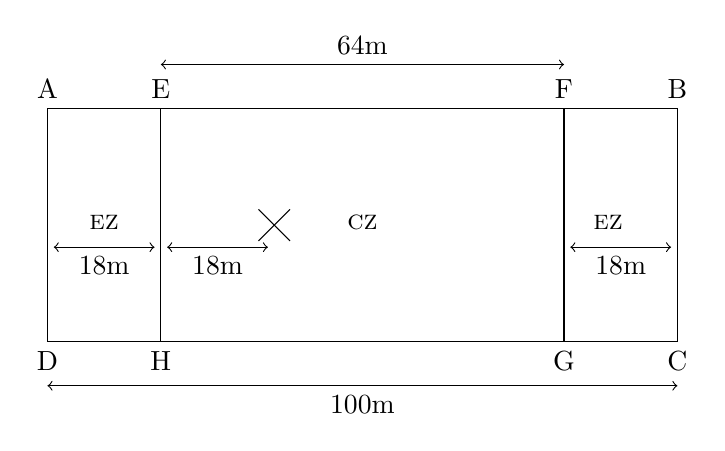
\begin{tikzpicture}[scale=0.08]
                              % Draw field outline
                              \draw (0,0) rectangle (100,37);

                              % Draw goal areas
                              \draw (0,0) rectangle (18,37);
                              \draw (82,0) rectangle (100,37);

                                % brick mark
                              \draw (33.5,16) -- (38.5,21);
                              \draw (38.5,16) -- (33.5,21);


                              % length arrows
                              \draw[<->] (0,-7) -- (100,-7) node[midway, below] {100m};
                              \draw[<->] (19,15) -- (35,15) node[midway, below] {18m};
                              \draw[<->] (1,15) -- (17,15) node[midway, below] {18m};
                              \draw[<->] (83,15) -- (99,15) node[midway, below] {18m};
                              \draw[<->] (18,44) -- (82,44) node[midway, above] {64m};


                              % labels
                              \node at (0,37) [above] {A};
                              \node at (18,37) [above] {E};
                              \node at (82,37) [above] {F};
                              \node at (100,37) [above] {B};
                              \node at (0,0) [below] {D};
                              \node at (18,0) [below] {H};
                              \node at (82,0) [below] {G};
                              \node at (100,0) [below] {C};

                                \node at (50,19) {\sc cz};
                                \node at (9,19) {\sc ez};
                                \node at (89,19) {\sc ez};
                            \end{tikzpicture}
                            \vspace*{-1cm}
                            \[\{AB, BC, CD, DA\} \not \subset \text{field}\]
                            \[\{EH, FG\} \not \subset \text{EZ}\]


                            \begin{center}[0]\end{center}
                        \end{minipage}
                    }
                    \vspace*{1cm}
                    \fbox{
                        \begin{minipage}[t][0.22\textheight]{\textwidth}
                            \small{
                                \begin{itemize}
                                    \item first to 15 wins
                                    \item gamelength = 100 minutes
                                    \item you can play with a minimum of 5 players
                                    \item half time at 8 points
                                    \item two timeouts per half. 75 seconds each$^\dagger$
                                \end{itemize}
                            }
                            \begin{center}[1]\end{center}
                        \end{minipage}
                    }
                \end{minipage}
            }
        \end{multicols}
    \end{minipage}
}


\begin{turn}{180}
\fbox{
    \begin{minipage}[t][0.49\paperheight]{0.94\textwidth}
        \begin{multicols}{2}
            \fbox{
                \begin{minipage}[t][0.45\textheight]{0.45\textwidth}
                    \fbox{
                        \begin{minipage}[t][0.22\textheight]{\textwidth}
                            \underline{\uppercase{the pull}}
                            \begin{itemize}
                                \item
                                \item
                                \item
                                \item
                                \item
                                \item
                            \end{itemize}
                            \begin{center}[a]\end{center}
                        \end{minipage}
                    }
                    \fbox{
                        \begin{minipage}[t][0.22\textheight]{\textwidth}
                            \underline{\uppercase{stall counting}}
                            \begin{itemize}
                                \item
                                \item
                                \item
                                \item
                                \item
                                \item
                            \end{itemize}
                            \begin{center}[b]\end{center}
                        \end{minipage}
                    }
                \end{minipage}
            }
            \fbox{
                \begin{minipage}[t][0.45\textheight]{0.45\textwidth}
                    \fbox{
                        \begin{minipage}[t][0.22\textheight]{\textwidth}
                            \underline{\uppercase{offsides}}
                            \begin{itemize}
                                \item
                                \item
                                \item
                                \item
                                \item
                                \item
                            \end{itemize}
                            \begin{center}[c]\end{center}
                        \end{minipage}
                    }
                    \fbox{
                        \begin{minipage}[t][0.22\textheight]{\textwidth}
                            \underline{\uppercase{stoppages}}
                            \begin{itemize}
                                \item
                                \item
                                \item
                                \item
                                \item
                                \item
                            \end{itemize}
                            \begin{center}[d]\end{center}
                        \end{minipage}
                    }
                \end{minipage}
            }
        \end{multicols}
    \begin{center}[4]\end{center}
    \end{minipage}
}
\end{turn}


\newpage

\newgeometry{top=0mm,bottom=10mm,right=0mm,left=0mm,includeheadfoot}

\begin{multicols}{3}
    \fbox{
        \begin{minipage}[t][0.95\paperheight]{1in}
            \centering{
            \includegraphics[width=0.8\linewidth]{img/foul.png}

            1. Foul

            \includegraphics[width=\linewidth]{img/violation.png}

            2. Violation

            \includegraphics[width=\linewidth]{img/mark-inf.png}

            12. Marking Infraction

            \includegraphics[width=0.8\linewidth]{img/timing.png}

            14. Timing Violation

            \includegraphics[width=0.6\linewidth]{img/offside.png}

            15. Offside

            \includegraphics[width=0.6\linewidth]{img/stoppage.png}

            18. Stoppage

            \includegraphics[width=\linewidth]{img/gender-w.png}

            20. Gender Women

            \includegraphics[width=\linewidth]{img/play-stop.png}

            21. Stop play
        }
        \end{minipage}
    }
    \fbox{
        \begin{minipage}[t][0.9\textheight]{0.35\textwidth}
            \fbox{
                \begin{minipage}[t][0.45\textheight]{\textwidth}
                    \begin{center}\underline{\uppercase{turnovers}}\end{center}
                    \begin{itemize}
                        \item
                        \item
                        \item
                        \item
                        \item
                        \item
                    \end{itemize}
                    \begin{center}[5]\end{center}
                \end{minipage}
            }
            \fbox{
                \begin{minipage}[t][0.45\textheight]{\textwidth}
                    \begin{center}\underline{\uppercase{fouls}}\end{center}
                    \begin{itemize}
                        \item
                        \item
                        \item
                        \item
                        \item
                        \item
                    \end{itemize}
                    \begin{center}[6]\end{center}
                \end{minipage}
            }
        \end{minipage}
    }
    \hspace*{1.7in}
    \fbox{
        \begin{minipage}[t][0.9\textheight]{0.35\textwidth}
            \fbox{
                \begin{minipage}[t][0.45\textheight]{\textwidth}
                    \begin{center}\underline{\uppercase{infractions}}\end{center}
                    \begin{itemize}
                        \item
                        \item
                        \item
                        \item
                        \item
                        \item
                    \end{itemize}
                    \begin{center}[7]\end{center}
                \end{minipage}
            }
            \fbox{
                \begin{minipage}[t][0.45\textheight]{\textwidth}
                    \begin{center}\underline{\uppercase{violations}}\end{center}
                    \small{	
                    (The nourishment of the person)
                    All in the world know the beauty of the beautiful, and in doing this they have (the idea of) what ugliness is; they all know the skill of the skilful, and in doing this they have (the idea of) what the want of skill is. So it is that existence and non-existence give birth the one to (the idea of) the other; that difficulty and ease produce the one (the idea of) the other; that length and shortness fashion out the one the figure of the other; that (the ideas of) height and lowness arise from the contrast of the one with the other; that the musical notes and tones become harmonious through the relation of one with another; and that being before and behind give the idea of one following another. \textbf{Therefore the sage manages affairs without doing anything, and conveys his instructions without the use of speech. All things spring up, and there is not one which declines to show itself; they grow, and there is no claim made for their ownership; they go through their processes, and there is no expectation (of a reward for the results). The work is accomplished, and there is no resting in it (as an achievement).}
The work is done, but how no one can see;
'Tis this that makes the power not cease to be.
                    }
                \begin{center}[8]\end{center}
                \end{minipage}
            }
        \end{minipage}
    }

\end{multicols}


\end{document}


